% Created by tikzDevice version 0.6.1 on 2011-08-03 09:51:01
% !TEX encoding = UTF-8 Unicode
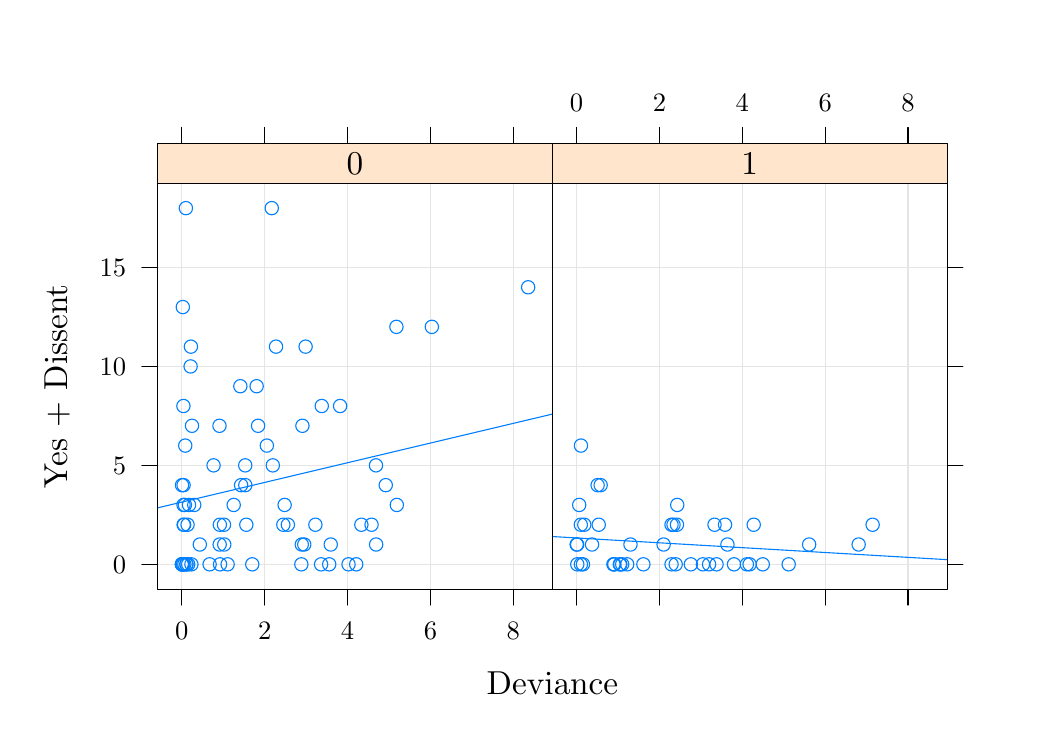
\begin{tikzpicture}[x=1pt,y=1pt]
\definecolor[named]{drawColor}{rgb}{0.00,0.00,0.00}
\definecolor[named]{fillColor}{rgb}{1.00,1.00,1.00}
\fill[color=fillColor,] (0,0) rectangle (361.35,252.94);
\begin{scope}
\path[clip] (  0.00,  0.00) rectangle (361.35,252.94);
\definecolor[named]{fillColor}{rgb}{0.00,0.00,0.00}
\end{scope}
\begin{scope}
\path[clip] (  0.00,  0.00) rectangle (361.35,252.94);
\definecolor[named]{fillColor}{rgb}{0.00,0.00,0.00}

\draw[fill opacity=0.00,draw opacity=0.00,] (  0.00,  0.00) rectangle (361.35,252.94);
\definecolor[named]{drawColor}{rgb}{0.00,0.00,0.00}

\node[color=drawColor,anchor=base,inner sep=0pt, outer sep=0pt, scale=  1.20] at (189.61, 12.04) {Deviance%
};
\end{scope}
\begin{scope}
\path[clip] (  0.00,  0.00) rectangle (361.35,252.94);
\definecolor[named]{fillColor}{rgb}{0.00,0.00,0.00}
\definecolor[named]{drawColor}{rgb}{0.00,0.00,0.00}

\node[rotate= 90.00,color=drawColor,anchor=base,inner sep=0pt, outer sep=0pt, scale=  1.20] at ( 14.29,123.38) {Yes + Dissent%
};
\end{scope}
\begin{scope}
\path[clip] (  0.00,  0.00) rectangle (361.35,252.94);
\definecolor[named]{fillColor}{rgb}{0.00,0.00,0.00}
\end{scope}
\begin{scope}
\path[clip] (  0.00,  0.00) rectangle (361.35,252.94);
\definecolor[named]{fillColor}{rgb}{0.00,0.00,0.00}
\end{scope}
\begin{scope}
\path[clip] (  0.00,  0.00) rectangle (361.35,252.94);
\definecolor[named]{fillColor}{rgb}{0.00,0.00,0.00}
\end{scope}
\begin{scope}
\path[clip] ( 46.98, 50.02) rectangle (189.61,196.74);
\definecolor[named]{fillColor}{rgb}{0.00,0.00,0.00}
\end{scope}
\begin{scope}
\path[clip] (  0.00,  0.00) rectangle (361.35,252.94);
\definecolor[named]{fillColor}{rgb}{0.00,0.00,0.00}
\end{scope}
\begin{scope}
\path[clip] (  0.00,  0.00) rectangle (361.35,252.94);
\definecolor[named]{fillColor}{rgb}{0.00,0.00,0.00}
\definecolor[named]{drawColor}{rgb}{0.00,0.00,0.00}

\draw[color=drawColor,line cap=round,line join=round,fill opacity=0.00,] ( 55.71,211.19) -- ( 55.71,216.88);

\draw[color=drawColor,line cap=round,line join=round,fill opacity=0.00,] ( 85.66,211.19) -- ( 85.66,216.88);

\draw[color=drawColor,line cap=round,line join=round,fill opacity=0.00,] (115.60,211.19) -- (115.60,216.88);

\draw[color=drawColor,line cap=round,line join=round,fill opacity=0.00,] (145.54,211.19) -- (145.54,216.88);

\draw[color=drawColor,line cap=round,line join=round,fill opacity=0.00,] (175.48,211.19) -- (175.48,216.88);
\end{scope}
\begin{scope}
\path[clip] (  0.00,  0.00) rectangle (361.35,252.94);
\definecolor[named]{fillColor}{rgb}{0.00,0.00,0.00}
\end{scope}
\begin{scope}
\path[clip] (  0.00,  0.00) rectangle (361.35,252.94);
\definecolor[named]{fillColor}{rgb}{0.00,0.00,0.00}
\definecolor[named]{drawColor}{rgb}{0.00,0.00,0.00}

\draw[color=drawColor,line cap=round,line join=round,fill opacity=0.00,] ( 46.98, 59.02) -- ( 41.29, 59.02);

\draw[color=drawColor,line cap=round,line join=round,fill opacity=0.00,] ( 46.98, 94.78) -- ( 41.29, 94.78);

\draw[color=drawColor,line cap=round,line join=round,fill opacity=0.00,] ( 46.98,130.53) -- ( 41.29,130.53);

\draw[color=drawColor,line cap=round,line join=round,fill opacity=0.00,] ( 46.98,166.28) -- ( 41.29,166.28);

\node[color=drawColor,anchor=base east,inner sep=0pt, outer sep=0pt, scale=  0.96] at ( 35.60, 55.72) {0%
};

\node[color=drawColor,anchor=base east,inner sep=0pt, outer sep=0pt, scale=  0.96] at ( 35.60, 91.47) {5%
};

\node[color=drawColor,anchor=base east,inner sep=0pt, outer sep=0pt, scale=  0.96] at ( 35.60,127.22) {10%
};

\node[color=drawColor,anchor=base east,inner sep=0pt, outer sep=0pt, scale=  0.96] at ( 35.60,162.97) {15%
};
\end{scope}
\begin{scope}
\path[clip] (  0.00,  0.00) rectangle (361.35,252.94);
\definecolor[named]{fillColor}{rgb}{0.00,0.00,0.00}
\end{scope}
\begin{scope}
\path[clip] (  0.00,  0.00) rectangle (361.35,252.94);
\definecolor[named]{fillColor}{rgb}{0.00,0.00,0.00}
\definecolor[named]{drawColor}{rgb}{0.00,0.00,0.00}

\draw[color=drawColor,line cap=round,line join=round,fill opacity=0.00,] ( 55.71, 50.02) -- ( 55.71, 44.32);

\draw[color=drawColor,line cap=round,line join=round,fill opacity=0.00,] ( 85.66, 50.02) -- ( 85.66, 44.32);

\draw[color=drawColor,line cap=round,line join=round,fill opacity=0.00,] (115.60, 50.02) -- (115.60, 44.32);

\draw[color=drawColor,line cap=round,line join=round,fill opacity=0.00,] (145.54, 50.02) -- (145.54, 44.32);

\draw[color=drawColor,line cap=round,line join=round,fill opacity=0.00,] (175.48, 50.02) -- (175.48, 44.32);

\node[color=drawColor,anchor=base,inner sep=0pt, outer sep=0pt, scale=  0.96] at ( 55.71, 32.02) {0%
};

\node[color=drawColor,anchor=base,inner sep=0pt, outer sep=0pt, scale=  0.96] at ( 85.66, 32.02) {2%
};

\node[color=drawColor,anchor=base,inner sep=0pt, outer sep=0pt, scale=  0.96] at (115.60, 32.02) {4%
};

\node[color=drawColor,anchor=base,inner sep=0pt, outer sep=0pt, scale=  0.96] at (145.54, 32.02) {6%
};

\node[color=drawColor,anchor=base,inner sep=0pt, outer sep=0pt, scale=  0.96] at (175.48, 32.02) {8%
};
\end{scope}
\begin{scope}
\path[clip] (  0.00,  0.00) rectangle (361.35,252.94);
\definecolor[named]{fillColor}{rgb}{0.00,0.00,0.00}
\end{scope}
\begin{scope}
\path[clip] ( 46.98, 50.02) rectangle (189.61,196.74);
\definecolor[named]{fillColor}{rgb}{0.00,0.00,0.00}
\definecolor[named]{drawColor}{rgb}{0.90,0.90,0.90}

\draw[color=drawColor,line cap=round,line join=round,fill opacity=0.00,] ( 46.98, 59.02) -- (189.61, 59.02);

\draw[color=drawColor,line cap=round,line join=round,fill opacity=0.00,] ( 46.98, 94.78) -- (189.61, 94.78);

\draw[color=drawColor,line cap=round,line join=round,fill opacity=0.00,] ( 46.98,130.53) -- (189.61,130.53);

\draw[color=drawColor,line cap=round,line join=round,fill opacity=0.00,] ( 46.98,166.28) -- (189.61,166.28);

\draw[color=drawColor,line cap=round,line join=round,fill opacity=0.00,] ( 55.71, 50.02) -- ( 55.71,196.74);

\draw[color=drawColor,line cap=round,line join=round,fill opacity=0.00,] ( 85.66, 50.02) -- ( 85.66,196.74);

\draw[color=drawColor,line cap=round,line join=round,fill opacity=0.00,] (115.60, 50.02) -- (115.60,196.74);

\draw[color=drawColor,line cap=round,line join=round,fill opacity=0.00,] (145.54, 50.02) -- (145.54,196.74);

\draw[color=drawColor,line cap=round,line join=round,fill opacity=0.00,] (175.48, 50.02) -- (175.48,196.74);
\definecolor[named]{drawColor}{rgb}{0.00,0.50,1.00}

\draw[color=drawColor,line cap=round,line join=round,fill opacity=0.00,] ( 58.00, 59.02) circle (  2.41);

\draw[color=drawColor,line cap=round,line join=round,fill opacity=0.00,] ( 58.30, 80.48) circle (  2.41);

\draw[color=drawColor,line cap=round,line join=round,fill opacity=0.00,] ( 59.17, 59.02) circle (  2.41);

\draw[color=drawColor,line cap=round,line join=round,fill opacity=0.00,] (125.86, 94.78) circle (  2.41);

\draw[color=drawColor,line cap=round,line join=round,fill opacity=0.00,] ( 60.19, 80.48) circle (  2.41);

\draw[color=drawColor,line cap=round,line join=round,fill opacity=0.00,] ( 92.38, 73.33) circle (  2.41);

\draw[color=drawColor,line cap=round,line join=round,fill opacity=0.00,] ( 70.94, 73.33) circle (  2.41);

\draw[color=drawColor,line cap=round,line join=round,fill opacity=0.00,] ( 55.79, 59.02) circle (  2.41);

\draw[color=drawColor,line cap=round,line join=round,fill opacity=0.00,] ( 56.21, 59.02) circle (  2.41);

\draw[color=drawColor,line cap=round,line join=round,fill opacity=0.00,] ( 56.64, 59.02) circle (  2.41);

\draw[color=drawColor,line cap=round,line join=round,fill opacity=0.00,] ( 69.31,109.08) circle (  2.41);

\draw[color=drawColor,line cap=round,line join=round,fill opacity=0.00,] ( 59.38,109.08) circle (  2.41);

\draw[color=drawColor,line cap=round,line join=round,fill opacity=0.00,] ( 56.81, 80.48) circle (  2.41);

\draw[color=drawColor,line cap=round,line join=round,fill opacity=0.00,] ( 57.40, 59.02) circle (  2.41);

\draw[color=drawColor,line cap=round,line join=round,fill opacity=0.00,] ( 89.74,137.68) circle (  2.41);

\draw[color=drawColor,line cap=round,line join=round,fill opacity=0.00,] (106.27,116.23) circle (  2.41);

\draw[color=drawColor,line cap=round,line join=round,fill opacity=0.00,] (103.97, 73.33) circle (  2.41);

\draw[color=drawColor,line cap=round,line join=round,fill opacity=0.00,] (106.03, 59.02) circle (  2.41);

\draw[color=drawColor,line cap=round,line join=round,fill opacity=0.00,] ( 56.94,101.93) circle (  2.41);

\draw[color=drawColor,line cap=round,line join=round,fill opacity=0.00,] ( 62.20, 66.18) circle (  2.41);

\draw[color=drawColor,line cap=round,line join=round,fill opacity=0.00,] ( 55.86, 59.02) circle (  2.41);

\draw[color=drawColor,line cap=round,line join=round,fill opacity=0.00,] ( 56.54, 73.33) circle (  2.41);

\draw[color=drawColor,line cap=round,line join=round,fill opacity=0.00,] ( 69.51, 59.02) circle (  2.41);

\draw[color=drawColor,line cap=round,line join=round,fill opacity=0.00,] ( 57.77, 73.33) circle (  2.41);

\draw[color=drawColor,line cap=round,line join=round,fill opacity=0.00,] ( 57.32, 59.02) circle (  2.41);

\draw[color=drawColor,line cap=round,line join=round,fill opacity=0.00,] (115.94, 59.02) circle (  2.41);

\draw[color=drawColor,line cap=round,line join=round,fill opacity=0.00,] (120.58, 73.33) circle (  2.41);

\draw[color=drawColor,line cap=round,line join=round,fill opacity=0.00,] (129.39, 87.63) circle (  2.41);

\draw[color=drawColor,line cap=round,line join=round,fill opacity=0.00,] ( 72.25, 59.02) circle (  2.41);

\draw[color=drawColor,line cap=round,line join=round,fill opacity=0.00,] ( 69.44, 73.33) circle (  2.41);

\draw[color=drawColor,line cap=round,line join=round,fill opacity=0.00,] ( 77.12, 87.63) circle (  2.41);

\draw[color=drawColor,line cap=round,line join=round,fill opacity=0.00,] ( 86.42,101.93) circle (  2.41);

\draw[color=drawColor,line cap=round,line join=round,fill opacity=0.00,] ( 57.17,187.73) circle (  2.41);

\draw[color=drawColor,line cap=round,line join=round,fill opacity=0.00,] (100.43,137.68) circle (  2.41);

\draw[color=drawColor,line cap=round,line join=round,fill opacity=0.00,] (146.05,144.83) circle (  2.41);

\draw[color=drawColor,line cap=round,line join=round,fill opacity=0.00,] ( 69.38, 66.18) circle (  2.41);

\draw[color=drawColor,line cap=round,line join=round,fill opacity=0.00,] ( 71.04, 66.18) circle (  2.41);

\draw[color=drawColor,line cap=round,line join=round,fill opacity=0.00,] ( 56.33, 87.63) circle (  2.41);

\draw[color=drawColor,line cap=round,line join=round,fill opacity=0.00,] ( 74.44, 80.48) circle (  2.41);

\draw[color=drawColor,line cap=round,line join=round,fill opacity=0.00,] (125.92, 66.18) circle (  2.41);

\draw[color=drawColor,line cap=round,line join=round,fill opacity=0.00,] ( 83.26,109.08) circle (  2.41);

\draw[color=drawColor,line cap=round,line join=round,fill opacity=0.00,] ( 55.78, 59.02) circle (  2.41);

\draw[color=drawColor,line cap=round,line join=round,fill opacity=0.00,] ( 55.74, 59.02) circle (  2.41);

\draw[color=drawColor,line cap=round,line join=round,fill opacity=0.00,] (124.26, 73.33) circle (  2.41);

\draw[color=drawColor,line cap=round,line join=round,fill opacity=0.00,] ( 88.58, 94.78) circle (  2.41);

\draw[color=drawColor,line cap=round,line join=round,fill opacity=0.00,] ( 99.94, 66.18) circle (  2.41);

\draw[color=drawColor,line cap=round,line join=round,fill opacity=0.00,] (108.96, 59.02) circle (  2.41);

\draw[color=drawColor,line cap=round,line join=round,fill opacity=0.00,] (109.51, 66.18) circle (  2.41);

\draw[color=drawColor,line cap=round,line join=round,fill opacity=0.00,] (118.72, 59.02) circle (  2.41);

\draw[color=drawColor,line cap=round,line join=round,fill opacity=0.00,] (133.39, 80.48) circle (  2.41);

\draw[color=drawColor,line cap=round,line join=round,fill opacity=0.00,] ( 65.74, 59.02) circle (  2.41);

\draw[color=drawColor,line cap=round,line join=round,fill opacity=0.00,] ( 92.85, 80.48) circle (  2.41);

\draw[color=drawColor,line cap=round,line join=round,fill opacity=0.00,] ( 55.77, 87.63) circle (  2.41);

\draw[color=drawColor,line cap=round,line join=round,fill opacity=0.00,] ( 55.80, 59.02) circle (  2.41);

\draw[color=drawColor,line cap=round,line join=round,fill opacity=0.00,] ( 81.15, 59.02) circle (  2.41);

\draw[color=drawColor,line cap=round,line join=round,fill opacity=0.00,] ( 56.28,116.23) circle (  2.41);

\draw[color=drawColor,line cap=round,line join=round,fill opacity=0.00,] ( 56.35, 73.33) circle (  2.41);

\draw[color=drawColor,line cap=round,line join=round,fill opacity=0.00,] ( 56.32, 80.48) circle (  2.41);

\draw[color=drawColor,line cap=round,line join=round,fill opacity=0.00,] ( 56.06,151.98) circle (  2.41);

\draw[color=drawColor,line cap=round,line join=round,fill opacity=0.00,] ( 78.61, 94.78) circle (  2.41);

\draw[color=drawColor,line cap=round,line join=round,fill opacity=0.00,] ( 58.87,130.53) circle (  2.41);

\draw[color=drawColor,line cap=round,line join=round,fill opacity=0.00,] ( 67.17, 94.78) circle (  2.41);

\draw[color=drawColor,line cap=round,line join=round,fill opacity=0.00,] ( 99.05, 66.18) circle (  2.41);

\draw[color=drawColor,line cap=round,line join=round,fill opacity=0.00,] ( 82.73,123.38) circle (  2.41);

\draw[color=drawColor,line cap=round,line join=round,fill opacity=0.00,] (180.85,159.13) circle (  2.41);

\draw[color=drawColor,line cap=round,line join=round,fill opacity=0.00,] (112.90,116.23) circle (  2.41);

\draw[color=drawColor,line cap=round,line join=round,fill opacity=0.00,] ( 99.28,109.08) circle (  2.41);

\draw[color=drawColor,line cap=round,line join=round,fill opacity=0.00,] ( 98.89, 59.02) circle (  2.41);

\draw[color=drawColor,line cap=round,line join=round,fill opacity=0.00,] ( 94.02, 73.33) circle (  2.41);

\draw[color=drawColor,line cap=round,line join=round,fill opacity=0.00,] (133.25,144.83) circle (  2.41);

\draw[color=drawColor,line cap=round,line join=round,fill opacity=0.00,] ( 79.01, 73.33) circle (  2.41);

\draw[color=drawColor,line cap=round,line join=round,fill opacity=0.00,] ( 58.98,137.68) circle (  2.41);

\draw[color=drawColor,line cap=round,line join=round,fill opacity=0.00,] ( 88.20,187.73) circle (  2.41);

\draw[color=drawColor,line cap=round,line join=round,fill opacity=0.00,] ( 76.85,123.38) circle (  2.41);

\draw[color=drawColor,line cap=round,line join=round,fill opacity=0.00,] ( 78.64, 87.63) circle (  2.41);

\draw[color=drawColor,line cap=round,line join=round,fill opacity=0.00,] (189.61,113.31) --
	( 46.98, 79.43);
\end{scope}
\begin{scope}
\path[clip] (  0.00,  0.00) rectangle (361.35,252.94);
\definecolor[named]{fillColor}{rgb}{0.00,0.00,0.00}
\end{scope}
\begin{scope}
\path[clip] (  0.00,  0.00) rectangle (361.35,252.94);
\definecolor[named]{fillColor}{rgb}{0.00,0.00,0.00}
\definecolor[named]{drawColor}{rgb}{0.00,0.00,0.00}

\draw[color=drawColor,line cap=round,line join=round,fill opacity=0.00,] ( 46.98, 50.02) rectangle (189.61,196.74);
\end{scope}
\begin{scope}
\path[clip] (  0.00,  0.00) rectangle (361.35,252.94);
\definecolor[named]{fillColor}{rgb}{0.00,0.00,0.00}
\end{scope}
\begin{scope}
\path[clip] (  0.00,  0.00) rectangle (361.35,252.94);
\definecolor[named]{fillColor}{rgb}{0.00,0.00,0.00}
\end{scope}
\begin{scope}
\path[clip] ( 46.98,196.74) rectangle (189.61,211.19);
\definecolor[named]{fillColor}{rgb}{0.00,0.00,0.00}
\definecolor[named]{drawColor}{rgb}{1.00,0.90,0.80}
\definecolor[named]{fillColor}{rgb}{1.00,0.90,0.80}

\draw[color=drawColor,line cap=round,line join=round,fill=fillColor,] ( 46.98,196.74) rectangle (189.61,211.19);
\definecolor[named]{drawColor}{rgb}{0.00,0.00,0.00}

\node[color=drawColor,anchor=base west,inner sep=0pt, outer sep=0pt, scale=  1.20] at (115.29,199.83) {0%
};
\end{scope}
\begin{scope}
\path[clip] (  0.00,  0.00) rectangle (361.35,252.94);
\definecolor[named]{fillColor}{rgb}{0.00,0.00,0.00}
\end{scope}
\begin{scope}
\path[clip] (  0.00,  0.00) rectangle (361.35,252.94);
\definecolor[named]{fillColor}{rgb}{0.00,0.00,0.00}
\definecolor[named]{drawColor}{rgb}{0.00,0.00,0.00}

\draw[color=drawColor,line cap=round,line join=round,fill opacity=0.00,] ( 46.98,196.74) rectangle (189.61,211.19);
\end{scope}
\begin{scope}
\path[clip] (  0.00,  0.00) rectangle (361.35,252.94);
\definecolor[named]{fillColor}{rgb}{0.00,0.00,0.00}
\end{scope}
\begin{scope}
\path[clip] (  0.00,  0.00) rectangle (361.35,252.94);
\definecolor[named]{fillColor}{rgb}{0.00,0.00,0.00}
\end{scope}
\begin{scope}
\path[clip] (189.61, 50.02) rectangle (332.23,196.74);
\definecolor[named]{fillColor}{rgb}{0.00,0.00,0.00}
\end{scope}
\begin{scope}
\path[clip] (  0.00,  0.00) rectangle (361.35,252.94);
\definecolor[named]{fillColor}{rgb}{0.00,0.00,0.00}
\end{scope}
\begin{scope}
\path[clip] (  0.00,  0.00) rectangle (361.35,252.94);
\definecolor[named]{fillColor}{rgb}{0.00,0.00,0.00}
\definecolor[named]{drawColor}{rgb}{0.00,0.00,0.00}

\draw[color=drawColor,line cap=round,line join=round,fill opacity=0.00,] (198.34,211.19) -- (198.34,216.88);

\draw[color=drawColor,line cap=round,line join=round,fill opacity=0.00,] (228.28,211.19) -- (228.28,216.88);

\draw[color=drawColor,line cap=round,line join=round,fill opacity=0.00,] (258.23,211.19) -- (258.23,216.88);

\draw[color=drawColor,line cap=round,line join=round,fill opacity=0.00,] (288.17,211.19) -- (288.17,216.88);

\draw[color=drawColor,line cap=round,line join=round,fill opacity=0.00,] (318.11,211.19) -- (318.11,216.88);

\node[color=drawColor,anchor=base,inner sep=0pt, outer sep=0pt, scale=  0.96] at (198.34,222.58) {0%
};

\node[color=drawColor,anchor=base,inner sep=0pt, outer sep=0pt, scale=  0.96] at (228.28,222.58) {2%
};

\node[color=drawColor,anchor=base,inner sep=0pt, outer sep=0pt, scale=  0.96] at (258.23,222.58) {4%
};

\node[color=drawColor,anchor=base,inner sep=0pt, outer sep=0pt, scale=  0.96] at (288.17,222.58) {6%
};

\node[color=drawColor,anchor=base,inner sep=0pt, outer sep=0pt, scale=  0.96] at (318.11,222.58) {8%
};
\end{scope}
\begin{scope}
\path[clip] (  0.00,  0.00) rectangle (361.35,252.94);
\definecolor[named]{fillColor}{rgb}{0.00,0.00,0.00}
\end{scope}
\begin{scope}
\path[clip] (  0.00,  0.00) rectangle (361.35,252.94);
\definecolor[named]{fillColor}{rgb}{0.00,0.00,0.00}
\end{scope}
\begin{scope}
\path[clip] (  0.00,  0.00) rectangle (361.35,252.94);
\definecolor[named]{fillColor}{rgb}{0.00,0.00,0.00}
\end{scope}
\begin{scope}
\path[clip] (  0.00,  0.00) rectangle (361.35,252.94);
\definecolor[named]{fillColor}{rgb}{0.00,0.00,0.00}
\definecolor[named]{drawColor}{rgb}{0.00,0.00,0.00}

\draw[color=drawColor,line cap=round,line join=round,fill opacity=0.00,] (198.34, 50.02) -- (198.34, 44.32);

\draw[color=drawColor,line cap=round,line join=round,fill opacity=0.00,] (228.28, 50.02) -- (228.28, 44.32);

\draw[color=drawColor,line cap=round,line join=round,fill opacity=0.00,] (258.23, 50.02) -- (258.23, 44.32);

\draw[color=drawColor,line cap=round,line join=round,fill opacity=0.00,] (288.17, 50.02) -- (288.17, 44.32);

\draw[color=drawColor,line cap=round,line join=round,fill opacity=0.00,] (318.11, 50.02) -- (318.11, 44.32);

\draw[color=drawColor,line cap=round,line join=round,fill opacity=0.00,] (332.23, 59.02) -- (337.92, 59.02);

\draw[color=drawColor,line cap=round,line join=round,fill opacity=0.00,] (332.23, 94.78) -- (337.92, 94.78);

\draw[color=drawColor,line cap=round,line join=round,fill opacity=0.00,] (332.23,130.53) -- (337.92,130.53);

\draw[color=drawColor,line cap=round,line join=round,fill opacity=0.00,] (332.23,166.28) -- (337.92,166.28);
\end{scope}
\begin{scope}
\path[clip] (  0.00,  0.00) rectangle (361.35,252.94);
\definecolor[named]{fillColor}{rgb}{0.00,0.00,0.00}
\end{scope}
\begin{scope}
\path[clip] (189.61, 50.02) rectangle (332.23,196.74);
\definecolor[named]{fillColor}{rgb}{0.00,0.00,0.00}
\definecolor[named]{drawColor}{rgb}{0.90,0.90,0.90}

\draw[color=drawColor,line cap=round,line join=round,fill opacity=0.00,] (189.61, 59.02) -- (332.23, 59.02);

\draw[color=drawColor,line cap=round,line join=round,fill opacity=0.00,] (189.61, 94.78) -- (332.23, 94.78);

\draw[color=drawColor,line cap=round,line join=round,fill opacity=0.00,] (189.61,130.53) -- (332.23,130.53);

\draw[color=drawColor,line cap=round,line join=round,fill opacity=0.00,] (189.61,166.28) -- (332.23,166.28);

\draw[color=drawColor,line cap=round,line join=round,fill opacity=0.00,] (198.34, 50.02) -- (198.34,196.74);

\draw[color=drawColor,line cap=round,line join=round,fill opacity=0.00,] (228.28, 50.02) -- (228.28,196.74);

\draw[color=drawColor,line cap=round,line join=round,fill opacity=0.00,] (258.23, 50.02) -- (258.23,196.74);

\draw[color=drawColor,line cap=round,line join=round,fill opacity=0.00,] (288.17, 50.02) -- (288.17,196.74);

\draw[color=drawColor,line cap=round,line join=round,fill opacity=0.00,] (318.11, 50.02) -- (318.11,196.74);
\definecolor[named]{drawColor}{rgb}{0.00,0.50,1.00}

\draw[color=drawColor,line cap=round,line join=round,fill opacity=0.00,] (211.98, 59.02) circle (  2.41);

\draw[color=drawColor,line cap=round,line join=round,fill opacity=0.00,] (262.35, 73.33) circle (  2.41);

\draw[color=drawColor,line cap=round,line join=round,fill opacity=0.00,] (234.72, 80.48) circle (  2.41);

\draw[color=drawColor,line cap=round,line join=round,fill opacity=0.00,] (214.15, 59.02) circle (  2.41);

\draw[color=drawColor,line cap=round,line join=round,fill opacity=0.00,] (198.57, 66.18) circle (  2.41);

\draw[color=drawColor,line cap=round,line join=round,fill opacity=0.00,] (198.38, 66.18) circle (  2.41);

\draw[color=drawColor,line cap=round,line join=round,fill opacity=0.00,] (198.60, 59.02) circle (  2.41);

\draw[color=drawColor,line cap=round,line join=round,fill opacity=0.00,] (246.22, 59.02) circle (  2.41);

\draw[color=drawColor,line cap=round,line join=round,fill opacity=0.00,] (203.93, 66.18) circle (  2.41);

\draw[color=drawColor,line cap=round,line join=round,fill opacity=0.00,] (199.93,101.93) circle (  2.41);

\draw[color=drawColor,line cap=round,line join=round,fill opacity=0.00,] (214.83, 59.02) circle (  2.41);

\draw[color=drawColor,line cap=round,line join=round,fill opacity=0.00,] (274.99, 59.02) circle (  2.41);

\draw[color=drawColor,line cap=round,line join=round,fill opacity=0.00,] (217.82, 66.18) circle (  2.41);

\draw[color=drawColor,line cap=round,line join=round,fill opacity=0.00,] (300.27, 66.18) circle (  2.41);

\draw[color=drawColor,line cap=round,line join=round,fill opacity=0.00,] (259.89, 59.02) circle (  2.41);

\draw[color=drawColor,line cap=round,line join=round,fill opacity=0.00,] (305.32, 73.33) circle (  2.41);

\draw[color=drawColor,line cap=round,line join=round,fill opacity=0.00,] (252.86, 66.18) circle (  2.41);

\draw[color=drawColor,line cap=round,line join=round,fill opacity=0.00,] (255.23, 59.02) circle (  2.41);

\draw[color=drawColor,line cap=round,line join=round,fill opacity=0.00,] (234.62, 73.33) circle (  2.41);

\draw[color=drawColor,line cap=round,line join=round,fill opacity=0.00,] (211.67, 59.02) circle (  2.41);

\draw[color=drawColor,line cap=round,line join=round,fill opacity=0.00,] (233.37, 73.33) circle (  2.41);

\draw[color=drawColor,line cap=round,line join=round,fill opacity=0.00,] (216.63, 59.02) circle (  2.41);

\draw[color=drawColor,line cap=round,line join=round,fill opacity=0.00,] (211.81, 59.02) circle (  2.41);

\draw[color=drawColor,line cap=round,line join=round,fill opacity=0.00,] (232.66, 59.02) circle (  2.41);

\draw[color=drawColor,line cap=round,line join=round,fill opacity=0.00,] (234.16, 59.02) circle (  2.41);

\draw[color=drawColor,line cap=round,line join=round,fill opacity=0.00,] (232.65, 73.33) circle (  2.41);

\draw[color=drawColor,line cap=round,line join=round,fill opacity=0.00,] (239.63, 59.02) circle (  2.41);

\draw[color=drawColor,line cap=round,line join=round,fill opacity=0.00,] (199.88, 73.33) circle (  2.41);

\draw[color=drawColor,line cap=round,line join=round,fill opacity=0.00,] (265.62, 59.02) circle (  2.41);

\draw[color=drawColor,line cap=round,line join=round,fill opacity=0.00,] (205.95, 87.63) circle (  2.41);

\draw[color=drawColor,line cap=round,line join=round,fill opacity=0.00,] (207.05, 87.63) circle (  2.41);

\draw[color=drawColor,line cap=round,line join=round,fill opacity=0.00,] (251.99, 73.33) circle (  2.41);

\draw[color=drawColor,line cap=round,line join=round,fill opacity=0.00,] (248.19, 73.33) circle (  2.41);

\draw[color=drawColor,line cap=round,line join=round,fill opacity=0.00,] (282.38, 66.18) circle (  2.41);

\draw[color=drawColor,line cap=round,line join=round,fill opacity=0.00,] (260.87, 59.02) circle (  2.41);

\draw[color=drawColor,line cap=round,line join=round,fill opacity=0.00,] (199.29, 80.48) circle (  2.41);

\draw[color=drawColor,line cap=round,line join=round,fill opacity=0.00,] (213.95, 59.02) circle (  2.41);

\draw[color=drawColor,line cap=round,line join=round,fill opacity=0.00,] (199.91, 59.02) circle (  2.41);

\draw[color=drawColor,line cap=round,line join=round,fill opacity=0.00,] (200.65, 59.02) circle (  2.41);

\draw[color=drawColor,line cap=round,line join=round,fill opacity=0.00,] (229.79, 66.18) circle (  2.41);

\draw[color=drawColor,line cap=round,line join=round,fill opacity=0.00,] (222.48, 59.02) circle (  2.41);

\draw[color=drawColor,line cap=round,line join=round,fill opacity=0.00,] (201.13, 73.33) circle (  2.41);

\draw[color=drawColor,line cap=round,line join=round,fill opacity=0.00,] (206.35, 73.33) circle (  2.41);

\draw[color=drawColor,line cap=round,line join=round,fill opacity=0.00,] (248.92, 59.02) circle (  2.41);

\draw[color=drawColor,line cap=round,line join=round,fill opacity=0.00,] (244.00, 59.02) circle (  2.41);

\draw[color=drawColor,line cap=round,line join=round,fill opacity=0.00,] (332.23, 60.71) --
	(189.61, 69.06);
\end{scope}
\begin{scope}
\path[clip] (  0.00,  0.00) rectangle (361.35,252.94);
\definecolor[named]{fillColor}{rgb}{0.00,0.00,0.00}
\end{scope}
\begin{scope}
\path[clip] (  0.00,  0.00) rectangle (361.35,252.94);
\definecolor[named]{fillColor}{rgb}{0.00,0.00,0.00}
\definecolor[named]{drawColor}{rgb}{0.00,0.00,0.00}

\draw[color=drawColor,line cap=round,line join=round,fill opacity=0.00,] (189.61, 50.02) rectangle (332.23,196.74);
\end{scope}
\begin{scope}
\path[clip] (  0.00,  0.00) rectangle (361.35,252.94);
\definecolor[named]{fillColor}{rgb}{0.00,0.00,0.00}
\end{scope}
\begin{scope}
\path[clip] (  0.00,  0.00) rectangle (361.35,252.94);
\definecolor[named]{fillColor}{rgb}{0.00,0.00,0.00}
\end{scope}
\begin{scope}
\path[clip] (189.61,196.74) rectangle (332.23,211.19);
\definecolor[named]{fillColor}{rgb}{0.00,0.00,0.00}
\definecolor[named]{drawColor}{rgb}{1.00,0.90,0.80}
\definecolor[named]{fillColor}{rgb}{1.00,0.90,0.80}

\draw[color=drawColor,line cap=round,line join=round,fill=fillColor,] (189.61,196.74) rectangle (332.23,211.19);
\definecolor[named]{drawColor}{rgb}{0.00,0.00,0.00}

\node[color=drawColor,anchor=base west,inner sep=0pt, outer sep=0pt, scale=  1.20] at (257.92,199.83) {1%
};
\end{scope}
\begin{scope}
\path[clip] (  0.00,  0.00) rectangle (361.35,252.94);
\definecolor[named]{fillColor}{rgb}{0.00,0.00,0.00}
\end{scope}
\begin{scope}
\path[clip] (  0.00,  0.00) rectangle (361.35,252.94);
\definecolor[named]{fillColor}{rgb}{0.00,0.00,0.00}
\definecolor[named]{drawColor}{rgb}{0.00,0.00,0.00}

\draw[color=drawColor,line cap=round,line join=round,fill opacity=0.00,] (189.61,196.74) rectangle (332.23,211.19);
\end{scope}
\begin{scope}
\path[clip] (  0.00,  0.00) rectangle (361.35,252.94);
\definecolor[named]{fillColor}{rgb}{0.00,0.00,0.00}
\end{scope}
\begin{scope}
\path[clip] (  0.00,  0.00) rectangle (361.35,252.94);
\definecolor[named]{fillColor}{rgb}{0.00,0.00,0.00}
\end{scope}
\begin{scope}
\path[clip] (  0.00,  0.00) rectangle (361.35,252.94);
\definecolor[named]{fillColor}{rgb}{0.00,0.00,0.00}
\end{scope}
\begin{scope}
\path[clip] (  0.00,  0.00) rectangle (361.35,252.94);
\definecolor[named]{fillColor}{rgb}{0.00,0.00,0.00}
\end{scope}
\end{tikzpicture}
